% !TEX program = xelatex
% 期刊/会议投稿版 —— 全六阶段，严格问题驱动
% 编译：xelatex main.tex （连续两次，以解析交叉引用）
\documentclass[11pt,a4paper]{ctexart}

\usepackage[a4paper,left=2.4cm,right=2.4cm,top=2.6cm,bottom=2.6cm]{geometry}
\usepackage{amsmath,amssymb,bm}
\usepackage{graphicx}
\usepackage{booktabs}
\usepackage{multirow}
\usepackage{makecell}
\usepackage{array}
\usepackage{caption}
\usepackage{enumitem}
\usepackage{xcolor}
\usepackage[hidelinks]{hyperref}
\usepackage{cleveref}
\usepackage{indentfirst}

\graphicspath{{../figures/}}
\captionsetup{font=small,labelfont=bf}
\setlength{\parindent}{2em}
\linespread{1.15}
\emergencystretch=2em
% cleveref 中文名（否则输出英文小写 "fig. 1" / "table 1"）
\crefname{figure}{图}{图}\Crefname{figure}{图}{图}
\crefname{table}{表}{表}\Crefname{table}{表}{表}
\crefname{equation}{式}{式}\Crefname{equation}{式}{式}
% 注意：不要给 section 设中文 crefname —— 会触发 "Extra \endcsname"。
% 章节引用一律写成「第 \ref{sec:xxx} 节」。


\newcommand{\alphahat}{\hat{\alpha}}
\newcommand{\dt}[2]{#1\,{\scriptstyle #2}}   % 维度标注

\title{\bfseries 逐层非线性失真下神经网络精度退化的成因\\[2pt] 读出瓶颈与双杠杆修复}
\author{黄奕皓\\[2pt] \small 中国科学院大学 计算机科学与技术，北京\\ \small \texttt{huangyihao24@mails.ucas.ac.cn}}
\date{}

\begin{document}
\maketitle

\vspace{-1.2em}
\begin{abstract}
\noindent
存算一体芯片的模拟域乘累加存在输入相关的非线性失真，通常建模为逐样本归一化后的三次多项式
$y=\alpha\hat{x}^3+(1-\alpha)\hat{x}$。本文在 CIFAR-10 与 CIFAR-100 上，用四个主干
（参数量 0.24M$\sim$11.2M）系统考察了这种失真的破坏形态、可达边界与修复路径。主要结论有四条。
\textbf{第一，灾难尾的瓶颈不在表征而在读出。} 在冻结主干的末端特征上重训线性探针，
$\alpha=+0.3$ 时可达 48.35\%，而模型自带分类头只有 28.09\%，headroom 为 20.26 个百分点；
同一套探针在加性高斯噪声这条对照通路上只有 7.50 个百分点。
\textbf{这条读数经四路主动加固}（随机标签、激活噪声下的临界崩塌点、划分与重采样、
以及与主干训练集完全不相交的划分），在最严口径下仍存活（$+16.23$，为规范口径的八成）；
它是\textbf{下界}——把探针样本加到 50000 后升至 $+27.63$（按不相交校正约 $+25.4$），且仍未饱和。
用三种非线性读出（k-NN 与两种 MLP）替换线性头，\textbf{没有一个能超过它}——容量不是这里的瓶颈。
\textbf{第二，因此最有效的修复动作在读出侧。}
冻结全部主干权重、只重训最后一个线性层（训练成本 12$\sim$30 分钟，为主干重训的 1/15$\sim$1/30），
尾部精度从 28.09/15.98/6.22 提升到 43.31/47.79/26.82（三个主干，各 3 个种子），
一致超过所有全网络鲁棒训练配方；而训练端的四条补救路径（采样预算分配、$\alpha$ 空间对抗训练、
课程式采样、训练范围外推至 $\pm0.5$）全部无效。
\textbf{第三，架构端存在一个与之正交的免费杠杆。} 把主干的最大池化层从 2 个增加到 5 个（不动训练脚本、参数量不变），
$\alpha=+0.3$ 从 28.09 提升到 42.47；机制上，这一保护主要来自降维而非池化算子本身——
三条独立的排除线（可交换性、不变区集中、max 的选择性）逐一否证了候选解释。
两个杠杆在尾部可叠加。此外，失真强度可由读出特征的岭回归在线恢复（$R^2$ 0.83$\sim$0.98），
使双头门控可以逼近 oracle；但门控有效需要两个前提同时成立，其边界由本文给出。
\textbf{第四，为一种失真做的鲁棒性训练不会顺带保护另一种。}
非线性与加性高斯之间的迁移近正交（但在 MaxPool 密集的 VGG-11 上被打破），
然而训练端存在\textbf{单向强干扰}——$\sigma$ 训练使 $\alpha$ 侧掉 6.08 个百分点，
联合训练使它掉 12.82；双扰动并存时的最优配方是 $\sigma$-only，不是联合训练。

最后，本文报告一条方法学结论：\textbf{跨训练实现比较精度数字会得到不可移植的结果}——
同一模型在两条评估路径下逐位相同，而两个训练脚本产出的权重稳定相差 5.55 个百分点，
该差异经三次干预实验仍未归因，按已知未知记录。
本文进一步把这个已知未知旁边的两级散布测准，给出一个\textbf{三级可分辨性}尺度
（种子噪声 / 过程自由度 / 跨实现），并表明\textbf{过程自由度的主要来源是"训多久"而非"用哪个优化器"}。

\vspace{0.6em}
\noindent\textbf{关键词：} 存算一体；非线性失真；读出瓶颈；有效秩；鲁棒性杠杆；测量纪律
\end{abstract}

\section{引言}

\subsection{问题}

在存算一体（Compute-in-Memory, CiM）架构中，乘累加运算在模拟域完成，
权重固化在存储阵列里~\cite{cim_survey,puma}。这消除了数据搬运开销，
但也把模拟器件的非理想特性直接引入了计算通路：器件失配、跨导放大器增益非线性、
工艺偏差与温度漂移，共同使输入-输出关系偏离理想的线性映射。
这一类误差有一个区别于常见扰动源的关键性质——它是\textbf{确定性的、且与输入幅度相关}的，
而不是像高斯噪声或随机 Dropout 那样零均值且与信号无关。

本文采用赛题给定的参数化模型：
\begin{equation}
y = \alpha\,\hat{x}^3 + (1-\alpha)\,\hat{x},
\qquad
\hat{x} = \frac{x}{\|x\|_\infty},
\label{eq:distortion}
\end{equation}
其中 $\hat{x}$ 按 batch 维\textbf{逐样本}做无穷范数归一化（避免样本间串扰），
失真通过前向钩子挂在每一个 \texttt{Conv2d} 与 \texttt{Linear} 算子的\textbf{输入侧}，
逐层注入。$\alpha$ 刻画非线性强度，$\alpha=0$ 退化为恒等映射；
$|\alpha|$ 越大失真越强，$\alpha$ 的符号决定失真的方向。

从工程角度看，这个问题的约束条件是硬的：\textbf{阵列里的权重不可重训}。
这既是 CiM 省功耗的前提，也意味着所有"重新训练网络以适应失真"的方案在部署阶段都不成立。
本文的出发点正是：在这个约束下，鲁棒性的杠杆究竟在哪里。

\subsection{本文的发现与贡献}

本文报告四条相互衔接的结论，以及一条方法学结论。

\begin{enumerate}[leftmargin=2em,itemsep=2pt]
  \item \textbf{定位}：灾难尾（$\alpha=+0.3$）损失的是读出的\textbf{可解码性}，而不是表征中的信息。
        直接用探针测量 headroom：$\alpha=+0.3$ 时为 20.26 个百分点，
        且随失真增强单调放大（$+0.4$ 时 30.90、$+0.5$ 时 30.82）。
        \textbf{这条读数经过四路主动加固}——随机标签、激活噪声下的临界崩塌点、
        划分与重采样、以及与主干训练集完全不相交的划分（见第 \ref{sec:probe} 节）；
        在最严口径下结论仍存活，幅度为规范口径的八成（$+16.23$）。
  \item \textbf{修复}：据此得到的读出适配方法（冻结主干、只重训线性读出——即迁移学习中的
        linear probing 一族）在三个主干上把尾部提升 13$\sim$23 个百分点，成本低 1$\sim$2 个数量级。
        \textbf{该做法本身不是本文的贡献}：当预训练特征好、偏移大时线性探针可胜过全量微调，
        这是已有理论与十数据集实证的结论（见第 \ref{sec:related} 节）；
        在存内计算领域，"冻结阵列、只在数字域补偿"也有先例，但那是标量或查找表级的校正。
        \textbf{本文的贡献是给出读出适配在本场景下的上界、机制与边界}，
        并指出在主干物理不可重训的约束下，它是唯一可行的一类修复。
        与之对照，训练端的四条独立路径全部失败，其中"把训练范围扩到 $\pm0.5$"这条
        最能说明问题的性质：模型在 $\alpha=+0.5$ 上仍只有 2.71\%，
        而同期负侧有 31.19\%。
  \item \textbf{第二个杠杆}：架构端的池化密度是一个与读出杠杆正交的、零训练成本的独立杠杆；
        其保护主要来自降维。两个杠杆在尾部可以叠加。
        本文据此给出一条\textbf{三步落地顺序}（第 \ref{sec:deploy} 节），
        并指出全部结论只依赖一个结构前提——读出层位于数字域或可重写。
  \item \textbf{失真通路的边界}：为一种失真做的鲁棒性训练\textbf{不会顺带保护另一种}。
        非线性与加性高斯之间的迁移近正交（但在 MaxPool 密集的 VGG-11 上被打破），
        然而训练端存在\textbf{单向强干扰}——$\sigma$ 训练使 $\alpha$ 侧掉 6.08 个百分点，
        联合训练使它掉 12.82；双扰动并存时的最优配方是 $\sigma$-only，不是联合训练。
  \item \textbf{方法学}：本文所有涉及深层主干或跨实现的比较都附带了方差标定与交叉评估，
        由此得到一条对同领域有直接约束力的结论——
        \textbf{同一份权重在不同评估路径下读数逐位相同，而不同训练脚本产出的权重稳定相差
        5.55 个百分点，且该差异经三次干预实验仍未归因}。
        这意味着跨实现引用精度数字是无效的。
        本文进一步把这个"已知未知"旁边的两级散布测准，给出一个\textbf{三级可分辨性}尺度
        （种子噪声 / 过程自由度 / 跨实现），并证明\textbf{过程自由度的主要来源是"训多久"
        而非"用哪个优化器"}（第 \ref{sec:variance} 节）。
\end{enumerate}

第 \ref{sec:method} 节给出方法与协议；第 \ref{sec:results} 节按科学问题组织结果；
第 \ref{sec:discussion} 节综合讨论；第 \ref{sec:limit} 节给出局限与未来工作。

\subsection{相关工作}
\label{sec:related}

非线性感知训练（NAT）把失真注入训练过程，让网络在失真分布内学习，
是在此之前的范式~\cite{nat}。本文的结果表明该类方法的收益严格限定在训练分布之内，
且不触及本文关心的正侧尾部（\cref{fig:extrapolation}）。

量化是 CiM 的另一条主要误差通路~\cite{quant}。本文考察了失真与量化联合作用的场景，
并复现了一个反直觉现象：在池化密集的架构上，低位量化反而提升失真下的精度，
其机理与随机抖动无关（\cref{fig:dithering}）。这与经典的非减性抖动理论~\cite{dither} 有本质区别。

架构层面，残差连接~\cite{resnet} 与深度可分离的深层纯前馈结构~\cite{vgg}
在本文的扰动下表现出显著不同的脆弱性；数据集为 CIFAR~\cite{cifar}。

\textbf{与本文方法最接近的一条已有结论。}
「冻结主干、只重训最后的线性层」（linear probing）与全量微调的对比，
在迁移学习里是一条有理论与大规模实证支撑的已知结论：
当预训练特征足够好、且分布偏移足够大时，\textbf{线性探针的分布外精度反而高于全量微调}
（在 10 个偏移数据集上平均 \textbf{ID 高 2\%、OOD 低 7\%}），原因是微调在学头的同时
\textbf{扭曲了底层特征}（feature distortion）~\cite{lpft}。
本文的读出适配属于同一族做法。\textbf{本文的贡献不在于此规律本身}，而在于：
① 把它搬到一个新场景——失真是确定性的、逐层累积的输入侧系统误差，
而非统计意义上的分布偏移；② 在该场景下主干\textbf{物理上不可重训}，故读出适配不是"更优选择"而是唯一选择；
③ 给出该场景特有的\textbf{上界}（探针 headroom 与可恢复量）、\textbf{机制}（有效秩塌陷）
与\textbf{边界}（门控的两前提）。

\textbf{与 CIM 数字域补偿的关系。}
在存内计算领域，「冻结阵列、只在数字域补偿」已有先例，但形态是\textbf{标量或查找表级}的校正：
例如用器件特定的电导漂移查找表配合自适应量化，在\textbf{不做片上训练}的前提下达到软件基线精度~\cite{mtjcal}。
本文动的对象不同——不是调一个缩放因子，而是\textbf{重训整个线性读出层}。
代价相应更大：它要求读出层位于数字域或可重写（见第 \ref{sec:limit} 节）。
换言之，已有工作回答的是"能不能用数字域的便宜手段把阵列误差压下去"，
本文回答的是"误差到底损伤了哪一层、损伤了多少、以及修复的边界在哪"。

\textbf{关于本文最依赖的测量手段。}
本文的中心结论建立在线性探针的读数上。这一手段近年正受到系统质疑：
\textbf{探针精度饱和并不意味着信息在场，探针失灵也不意味着信息不在场}——
已有工作报告过探针精度 0.871、有效秩指标全部健康的表征，
在检索任务上却只恢复了 14.4 bit 中的 \textbf{0.00} bit，
作者因此警告「秩、探针与其他指标都可能在无支撑的评测上虚假饱和」~\cite{gjepa}。
本文对此的处理是\textbf{主动加固}：为探针读数配第二读法（激活噪声下的临界崩塌点）与多组对照，
详见第 \ref{sec:probe} 节与第七阶段的审计记录。

\section{方法}
\label{sec:method}

\subsection{度量口径}

全阶段统一使用四个标量指标，定义如下：

\begin{center}
\begin{tabular}{ll}
\toprule
指标 & 定义 \\
\midrule
\texttt{clean} & $\alpha=0$ 时的测试精度 \\
\texttt{drop@0.3} & \texttt{clean} 减去 $\alpha=+0.3$ 时的精度 \\
\texttt{mid\_band} & $\alpha\in\{-0.2,-0.1,+0.1,+0.2\}$ 四点的平均精度 \\
\texttt{mean7} & $\{-0.3,-0.2,-0.1,0,+0.1,+0.2,+0.3\}$ 七点的平均精度 \\
\bottomrule
\end{tabular}
\end{center}

\textbf{评估协议}固定为：全量测试集（10\,000 张）、best 权重、纯推理。
每个实验的强度扫描文件里 $\alpha=0$ 的行必须等于同目录 \texttt{metrics.json} 的
\texttt{best\_test\_acc}（容限 0.01）。这个自检结果记在全局台账的 \texttt{pairing\_check} 列中。
本论文引用的 152 行数据全部通过该自检，无一行错位。

\textbf{种子纪律}：凡涉及尾部指标的比较均使用 $\ge 3$ 个种子；
单种子的尾部差值小于 3 个百分点不作为结论（理由见第 \ref{sec:variance} 节）。

\subsection{数据集、主干与协议}

数据集为 CIFAR-10（10 类）与 CIFAR-100（100 类）。
四个主干及其参数量见表 \ref{tab:arch}。所有主干均在干净条件下训练 100$\sim$200 个 epoch，
优化器为 SGD（动量 0.9、权重衰减 $10^{-4}$），余弦退火调度。

\begin{table}[t]
\centering
\caption{主干与参数量（按类别数分列）。}
\label{tab:arch}
\small
\begin{tabular}{lccc}
\toprule
主干 & 参数量（CIFAR-10 / CIFAR-100） & 卷积层数 & MaxPool 数 \\
\midrule
SimpleCNN & 242\,474 / 254\,084 & 4 & 2 \\
SimpleCNN+3$\times$MaxPool & 242\,474 / 254\,084 & 4 & 5 \\
VGG-11 & 9\,231\,114 / 9\,277\,284 & 8 & 5 \\
ResNet-18 & 11\,173\,962 / 11\,220\,132 & 17 & 0 \\
\bottomrule
\end{tabular}
\end{table}

\textbf{失真注入}：逐层、逐样本，同一个 $\alpha$ 施加到所有层（除非特别说明）。
训练时的 $\alpha$ 采样区间为 $U[-0.3,+0.3]$，采样粒度在正文中注明。

\subsection{读出适配方法}

本文的主要方法（下称 readout-NAT）极为简单：\textbf{主干全部冻结}——
把主干参数的梯度开关全部关闭、一个参数都不更新——只重训最后那个
\texttt{nn.Linear} 分类头，训练数据为在 $\alpha\sim U[\pm0.3]$ 上采样的失真样本，
评估仍在干净与各 $\alpha$ 点上进行。默认配置为 24 个 epoch、20\,000 个特征样本。
对 SimpleCNN 而言读出层占全模型参数的 5.04\%，对 VGG-11 为 0.55\%。

\subsection{其他探针}

\textbf{信息探针}：在冻结主干的末端特征上重训一个线性分类器，与模型自带头比较，
差值记为 headroom。\textbf{秩探针}：对末端特征做 SVD，有效秩定义为
$\exp(-\sum_i p_i \ln p_i)$，其中 $p_i$ 为归一化奇异值；
同时记录 99\% 能量条件数 $\kappa_{99}$ 与 Fisher 判别比。
\textbf{交叉评估}：把 A 脚本训出的权重在 B 脚本的评估函数下扫描，反之亦然，
两条路径均从各自脚本原样导入，不复制、不改写。

\section{结果}
\label{sec:results}

\subsection{正向失真更致命，且这个方向性跨架构稳定——但倍数不是常数}

\cref{fig:direction} 给出三个主干在 CIFAR-100 上的七点扫描。
$\alpha>0$（正侧）的破坏力显著大于 $\alpha<0$（负侧），
且随容量与深度单调放大：$\alpha=+0.3$ 时 SimpleCNN 从 59.99 掉到 28.09，
VGG-11 从 67.09 掉到 16.92，ResNet-18 从 72.09 掉到 2.70。
按容量排序，\texttt{clean} 越高、\texttt{drop@0.3} 越大，这条反相关关系在同数据集内跨容量单调。

\begin{figure}[t]
\centering
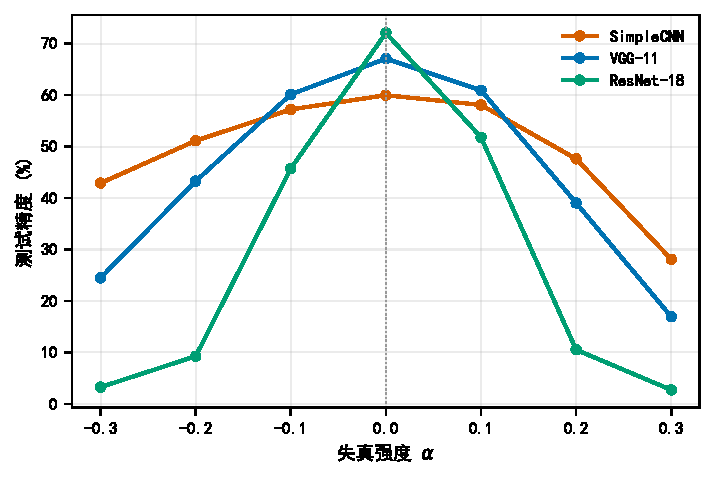
\includegraphics[width=0.72\textwidth]{F01_direction.pdf}
\caption{失真的方向性与容量依赖。三个主干在 CIFAR-100 上的七点扫描；
全量测试集、best 权重、纯推理。正侧（$\alpha>0$）的跌落显著大于负侧，
且跌幅随主干容量与深度单调增大。数据：\texttt{outputs\_cifar100/task1\_*/alpha\_sensitivity.csv}。}
\label{fig:direction}
\end{figure}

把"最脆弱的位置"进一步区分为\textbf{注入位置}与\textbf{观测位置}后，
一个反直觉的结果出现：在单层注入的探针中，最敏感的是中间层的卷积
（conv2 跌幅 $-12.43$、conv3 $-7.56$），而一直被当作瓶颈的 fc 层单点注入只有 $-0.68$。
全 5 层同时注入时跌幅 31.90，而按单层跌幅线性累加只有 23.33，超加性达 $-8.57$。
也就是说，损伤在层间\textbf{超加性累积}，而 fc 是误差的汇聚与观测点，不是注入敏感点。

需要强调的是，$\alpha>0$ 与 $\alpha<0$ 的破坏力之比\textbf{不是常数}：
在 CIFAR-10/SimpleCNN/$|\alpha|=0.3$ 这一个点上是 3.4，
而 CIFAR-100 的同一模型上只有 1.87。跨条件引用这个倍数会出错；
跨阶段稳定成立的只有\textbf{方向}。

\subsection{灾难尾丢的不是信息，而是读出的可解码性}
\label{sec:probe}

这是全文的枢纽。若正侧尾部是表征被摧毁，那么任何修复都必须改动主干；
若信息仍在、只是读不出来，则杠杆在读出侧。
\cref{fig:probe} 用探针把两者分开：在\textbf{冻结主干}的末端特征上重训线性分类器，
与模型自带分类头在同一条件下比较。

\begin{figure}[t]
\centering
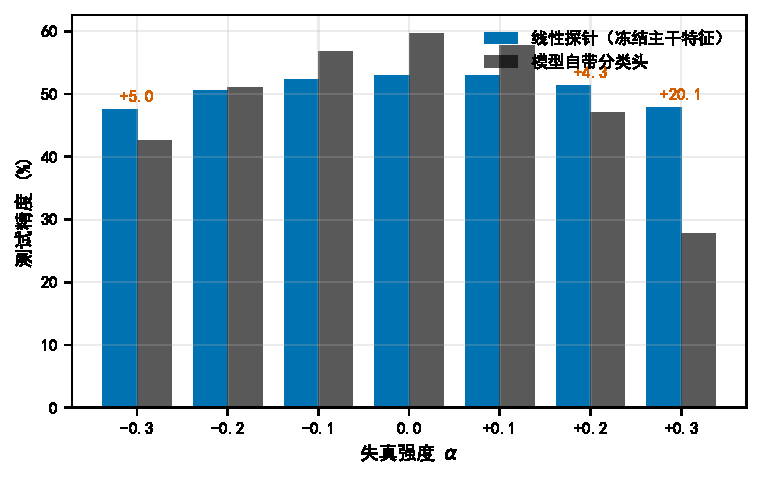
\includegraphics[width=0.78\textwidth]{F02_probe_headroom.pdf}
\caption{灾难尾的标签信息仍然线性可达。在同一冻结主干的末端特征上，
线性探针（实心）与模型自带分类头（空心）的精度对比；7 个 $\alpha$ 点，
CIFAR-100 \textbf{全量测试集}（10\,000 张）、best 权重、单种子。
$\alpha=+0.3$ 时两者相差 20.26 个百分点，且该差距随失真增强而放大。
作为对照，同一套探针在加性高斯噪声（$\sigma=0.3$）上只有 7.50 个百分点。
数据：\texttt{outputs\_cifar100/v7\_probe\_audit/ra\_onprotocol\_main.csv}。}
\label{fig:probe}
\end{figure}

$\alpha=+0.3$ 时探针达 48.35\%，自带头只有 28.09\%，headroom 为 \textbf{20.26} 个百分点%
\footnote{两项均取自\textbf{全量测试集}（10\,000 张），并与项目的规范口径逐位一致：
冻结头在 $\alpha=+0.3$ 的 28.09 等于 \texttt{task1} 扫描的同名行，
清洁模型在 $\alpha=0$ 的 59.99 等于 \texttt{metrics.json} 的 \texttt{best\_test\_acc}。
（早期版本的探针表曾用 8000 样本子集，给出 27.76 / 59.60 与 headroom $+20.12$；
第七阶段 M0c 已在同一设备上重跑全量口径并替换，全案见 \texttt{docs/IMPL\_AUDIT.md}。）}；
$\alpha=+0.4$ 时 30.90、$\alpha=+0.5$ 时 30.82。
失真越强，headroom 越大——这与"信息差被拉大"一致，而与"信息被摧毁"不一致。

\textbf{对照通路给出了这条测量的分辨力}：同样的探针在加性高斯噪声 $\sigma=0.3$ 下
headroom 只有 7.50 个百分点。随机扰动与确定性系统误差在"信息还剩多少"这个量上
清楚地分开，说明"先测 headroom"这个动作本身有判别价值。

\subsection{这条探针读数可信吗：一次主动加固}

上面那个 headroom 是\textbf{单点}探针读数，而线性探针近年正受到系统质疑：
探针精度饱和并不意味着信息在场，探针失灵也不意味着信息不在场；
已有工作报告过探针精度 0.871、有效秩指标全部健康的表征，
在检索任务上却只恢复了 14.4 bit 中的 \textbf{0.00} bit（见第 \ref{sec:related} 节）。
本文因此做了一组主动加固，四路对照如下。

\paragraph{对照一：随机标签。}
把探针的训练标签打乱后重训。9 个条件全部落在 $[0.85,1.11]\%$，
而 CIFAR-100 的随机水平是 $1.0\%$，\textbf{最大偏离 0.15 个百分点}。
⇒ 探针管线没有泄漏。

\paragraph{对照二：fragility（激活噪声下的临界崩塌点）。}
单点精度之外再取一个读数：给评估侧的激活加噪，测"探针精度跌到半程时的噪声水平" $\sigma^*$。
（噪声只加在\textbf{评估}侧——训练侧也加噪测的是解码器的抗噪补偿能力，是另一个量。）
结果：$\sigma^*$ 从 clean 的 \textbf{0.4188} 单调降到 $\alpha=+0.5$ 的 \textbf{0.1221}（$-71\%$），
\textbf{而负侧平缓得多}（0.3852 $\to$ 0.3310，仅 $-14\%$）。
这个正负不对称与 headroom 的不对称\textbf{同向}（$\alpha=+0.3$ 的 headroom 为 $+20.26$，
而 $\alpha=-0.3$ 仅 $+4.76$），两条独立的读数互相印证。

\paragraph{⚠ 这里有一个必须避开的陷阱，我们在本项目内实测到了它。}
$\sigma^*$ 的\textbf{单位}是关键：若用\textbf{绝对}噪声水平，会得出\textbf{符号相反}的结论：

\begin{center}
\small
\begin{tabular}{lccc}
\toprule
$\alpha$ & 激活 RMS & 绝对 $\sigma^*$ vs clean & \textbf{RMS 归一} $\sigma^*$ vs clean \\
\midrule
clean & 2.166 & --- & --- \\
$-0.3$ & \textbf{4.055}（$1.87\times$） & $+48\%$（\textbf{显得更鲁棒}） & $-21\%$（\textbf{更脆弱}） \\
$+0.3$ & 0.914（$0.42\times$） & $-67\%$（更脆弱） & $-23\%$（更脆弱） \\
\bottomrule
\end{tabular}
\end{center}

原因：$\alpha<0$ 把深层激活的幅度\textbf{抬高到 1.87 倍}，固定绝对噪声相对就更"小"，于是失真组
\textbf{虚假地显得更鲁棒}。归一化到该条件自身的 RMS 之后符号才正确。
⇒ \textbf{负侧的结论完全依赖这一步归一化}。本文一律使用 RMS 归一化的 $\sigma^*$，
并在 $\alpha\in\{+0.1,\dots,+0.5\}$ 上按逐对变化方向计票（10 对中 9 对反向），
确认它与 headroom 的结构一致，而非相反。

\paragraph{对照三与四：划分与不相交性。}
换 decoder 的随机种子与训练/测试划分（5 个划分 + 3 次 bootstrap）：读数稳定，
划分间标准差 0.14$\sim$1.33，bootstrap $\le$0.38。
更强的一项是把探针的训练与评估都放在\textbf{与主干训练集完全不相交}的样本上：
$\alpha=+0.3$ 的 headroom 为 $\bm{+16.23}$，即规范口径 $+20.26$ 的 \textbf{80\%}。

\paragraph{小结。}
四路对照都指向同一个方向：\textbf{headroom 这个结论在更严的口径下存活，但幅度会缩水到约八成}。
我们把它作为本文中心结论的\textbf{下界}：即使在"探针从没见过的样本上训练"这一最严设定下，
$\alpha=+0.3$ 处仍有一个约 16 个百分点的可解码性缺口。

\paragraph{而且这个缺口不是"线性读出"的假象。}
上面用的全是\textbf{线性}读出，所以"瓶颈在读出"有一个明显的反驳：
也许瓶颈只是在线性。为排除它，在同一批冻结特征上比较六种读出（$\alpha=+0.3$，CIFAR-100）：

\begin{center}
\small
\begin{tabular}{lcc}
\toprule
读出 & 精度 & 相对线性（同族公平锚） \\
\midrule
逻辑回归，强 L2（$C=0.01$） & 49.23 & $-2.24$ \\
逻辑回归（sklearn 默认，跨优化器参考臂） & 48.25 & $-3.22$ \\
k-NN（$k=20$） & 38.12 & $-13.35$ \\
\textbf{线性头（torch，公平锚）} & \textbf{51.47} & --- \\
瓶颈 MLP（$128\to32\to100$） & 43.38 & $-8.09$ \\
两层 MLP（$128\to256\to100$） & 48.62 & $-2.85$ \\
\bottomrule
\end{tabular}
\end{center}

\textbf{三种非线性读出没有一个超过线性头}，而且差距远超本文立的可分辨门槛
（$\Delta_{\text{proc}}=3.45$ pp，见第 \ref{sec:variance} 节）。
\textbf{参数越多反而越差}（瓶颈 MLP 43.38 $<$ 两层 MLP 48.62 $<$ 线性 51.47），
是典型的过拟合序（$n=8000$、100 类）。
⇒ 「\textbf{信息仍线性可达}」这句话，从"只测过线性"升级为
「\textbf{测过 k-NN 与两种 MLP 之后，线性头仍是最优读出}」。
\textbf{容量不是这里的瓶颈。}
（出处：\texttt{outputs\_cifar100/v7\_readout\_capacity/capacity\_ladder.csv}；
两个 torch 臂各在自己的最优轮数上取值，取值已记在产物里。）

\paragraph{这个下界还可以再抬高：headroom 依赖读出怎么训。}
上面四路对照都在\textbf{同一个探针设定}（$n=8000$ 训练样本）下做。
把探针的训练样本加到 50000（训练集全量），$\alpha=+0.3$ 的探针精度从 48.35 升到 \textbf{55.72}，
headroom 从 $+20.26$ 升到 \textbf{$+27.63$}——\textbf{且仍未饱和}
（对数刻度斜率只从 3.23 降到 2.71）。按第 \ref{sec:probe} 节的"不相交划分"校正（约 $-2.2$）
折合约 \textbf{$+25.4$}，\textbf{仍远高于 $+20.26$}。
clean 端也更清楚：$n=8000$ 时探针比冻结头低 6.42，$n=50000$ 时只低 \textbf{0.99}。

\textbf{这条观测的含义比数字本身重要}：$+20.26$ 不是表征的某个固定属性，
\textbf{它是"探针只喂了 8000 个样本"下的读数}。
⇒ \textbf{headroom 是读出训练方式的函数}——与第 \ref{sec:variance} 节那条
"过程自由度 3.45 pp"是同一件事的两个侧面，都指向同一个判断：
\textbf{读出这一层不是免费的，它的读数取决于你训得多好}。
本文因此把 $+20.26$ 作为\textbf{已审计的规范值}引用，同时声明它是\textbf{下界}；
真实可解码性\textbf{至少}为 $+25.4$。

（出处：\texttt{outputs\_cifar100/v7\_readout\_samplesize/samplesize\_ext.csv}。
$n=50000$ 档三个种子的标准差为 0——该档即训练集全量，各 seed 用同一批数据，故无采样变异。）

\subsection{冻结主干、只重训线性读出，就能以两个数量级更低的成本拿回尾部}

\cref{fig:readoutnat} 给出读出适配在三个主干上的效果。

\begin{figure}[t]
\centering
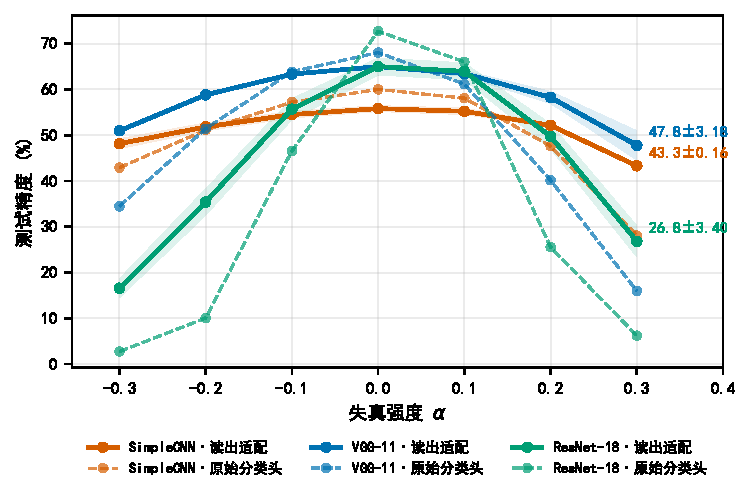
\includegraphics[width=0.76\textwidth]{F03_readout_nat.pdf}
\caption{读出适配跨三个主干一致抬升尾部。实线为 readout-NAT（冻结主干、只重训线性读出，
可训练参数占全模型 5.04\%/0.55\%），虚线为各模型自带的分类头；
每个主干为 3 个种子的逐点均值。$\alpha=+0.3$ 处的标注为均值$\pm$总体标准差。
数据：\texttt{outputs\_cifar100/v3\_readout\_repair/*ep24*.csv}。}
\label{fig:readoutnat}
\end{figure}

\begin{table}[t]
\centering
\caption{读出适配与全网络鲁棒训练的对照（CIFAR-100，$\alpha=+0.3$，精度 \%）}
\label{tab:nat}
\small
\begin{tabular}{lccccc}
\toprule
方法 & 可训练参数 & 训练成本 & SimpleCNN & VGG-11 & ResNet-18 \\
\midrule
干净模型（不处理） & --- & --- & 28.09 & 16.92 & 2.70 \\
本文读出适配（24ep，3 seed） & 12.8k / 51.2k & 12$\sim$30 min & \textbf{43.31}$\pm$0.16 & \textbf{47.79}$\pm$3.18 & \textbf{26.82}$\pm$3.40 \\
\midrule
全网络鲁棒训练（最好） & 全部 & 1$\sim$6.5 h & 26.57 & 24.69 & 6.22 \\
\bottomrule
\end{tabular}
\end{table}

\cref{tab:nat} 把两类方法并列。读出适配在三个主干上一致地超过"全网络重训"这一整类配方，
而可训练参数只有 5.04\%/0.55\%，训练时间低 1$\sim$2 个数量级。
代价是干净精度下降 3.19$\sim$6.67 个百分点——这一点在第 \ref{sec:gating} 节里被处理。

一个必要的自我校验：\textbf{读出适配不是"再分配"。}
把读出专门拟合到 $\alpha=+0.3$ 单点，该点确实从 28.09 涨到 52.79（$+24.70$），
但干净精度掉 20.36、$\alpha=-0.3$ 掉 25.71，七点均值反而低于基线。
而起作用的这一版是在 $\alpha\sim U[\pm0.3]$ 上分布的——它在每个扫描点都不显著劣化，
尾部与中带同时提升。同一层参数、两种训练方式给出质上不同的结果，
说明起作用的不是"读出被放开了"这件事本身。

\textbf{第二项自我校验：增益不是"多训了一个分类器"的通用效应。}
读出适配的全部改动只有最后一层。一个自然的怀疑是：任何重训过的线性头都会带来类似增益，
与"在哪种分布上训练"无关。\textbf{这个对照本来就在数据里}——
\texttt{v3\_readout\_repair} 的产物文件里每个权重都带有多个读出臂，
其中 \texttt{b\_clean\_fit\_linear} 是\textbf{在干净分布上重训同一个线性头}：

\begin{center}
\small
\begin{tabular}{llcccc}
\toprule
主干 & 原始头 & \textbf{在干净分布上重训} & $\Delta$ & 本文方法 & $\Delta$ \\
\midrule
SimpleCNN & 28.09 & \textbf{28.35} & $+0.26$ & 43.31 & $+15.22$ \\
VGG-11 & 15.98 & \textbf{15.81} & $-0.17$ & 47.79 & $+31.81$ \\
ResNet-18 & 6.22 & \textbf{5.38} & $-0.84$ & 26.82 & $+20.60$ \\
\bottomrule
\end{tabular}
\end{center}

（$\alpha=+0.3$ 精度，CIFAR-100，各 3 seed，24 epoch 读出；
出处：\texttt{outputs\_cifar100/v3\_readout\_repair/*ep24*.csv} 的 \texttt{a\_original\_fc}
与 \texttt{b\_clean\_fit\_linear} 两行。\textbf{表中为 3 个种子的均值}——
CSV 存的是逐 seed 的行，均值需自行合成，算式登记在 \texttt{docs/DERIVED\_VALUES.md}。）

\textbf{b 在三个主干上全部零增益，其中两个还是负的}（$+0.26$ / $-0.17$ / $-0.84$）。
⇒ 起作用的不是"换了一个头"，而是\textbf{头是在哪种分布上训练的}。

（同一批文件里还有一个 \texttt{c\_dist\_fit\_linear} 臂——把读出拟合到失真的窄分布上。
它在 $\alpha=+0.3$ 上更高（52.16 / 58.98 / 47.40，同为主干内 3 seed 均值），但\textbf{干净精度崩掉}：
ResNet-18 从 72.69 掉到 \textbf{15.53}。这是"再分配"的极端形态，也正是本文方法选择
在整个 $\alpha\sim U[\pm0.3]$ 区间上训练的原因。
\textbf{注意}：该臂是 24\,ep / 3 seed 口径，与上文引用的单点适配读数 52.79 来自不同轮次，
两者\textbf{不可直接相比}。）

\paragraph{同一套做法在更简单的任务上更强——一条标度律。}
把读出适配原样搬到 CIFAR-10（10 类，比 CIFAR-100 容易）：

\begin{center}
\small
\begin{tabular}{lcccccc}
\toprule
主干 & 原头 @$+0.3$ & 读出适配 @$+0.3$ & clean 代价 & \textbf{恢复率（C10）} & 恢复率（C100） \\
\midrule
SimpleCNN & 55.08 & \textbf{72.51} & $-0.84$ & \textbf{85.4\%} & 72.2\% \\
VGG-11 & 36.71 & \textbf{79.64} & $-0.58$ & \textbf{88.7\%} & 70.2\% \\
ResNet-18 & 17.09 & \textbf{44.37} & $-0.71$ & \textbf{48.2\%} & 36.9\% \\
\bottomrule
\end{tabular}
\end{center}

（24 epoch 读出，全量测试集；恢复率 $=$ 读出适配 @$+0.3$ 的精度 $\div$ 原头 @$\alpha=0$ 的精度。
CIFAR-100 的对应值取自 \cref{fig:rankrec} 所在小节。出处：\texttt{outputs/v3\_readout\_repair/*ep24*.csv}
与 \texttt{outputs\_cifar100/v3\_readout\_repair/*ep24*.csv}。）

两件事同时成立：\textbf{恢复率在三个主干上一致更高}（85.4 / 88.7 / 48.2 对 72.2 / 70.2 / 36.9），
\textbf{干净代价也小得多}（$-0.58\sim-0.84$ 对 $-3.19\sim-6.67$）。
⇒ 读出适配的收益\textbf{随"可用头部空间"缩放}：任务越难，能被读出捞回来的越少。
这与本文第 \ref{sec:probe} 节的逻辑一致——可恢复量由"信息还剩多少"决定，
而更难的任务在同样的失真下损耗更多。
（注：CIFAR-10 侧的读出为\textbf{单 seed}；CIFAR-100 侧为 3 seed。这一点记在局限里。）

\subsection{训练端的四条补救路径全部失效，因为损伤落在参数空间之外}

如果尾部是"训练不够适应"，那么更聪明的采样或更宽的分布应该能救它。
\cref{fig:training} 给出四条独立路径的结果，全部在同一 harness 下与均匀采样基准对比。

\begin{figure}[t]
\centering
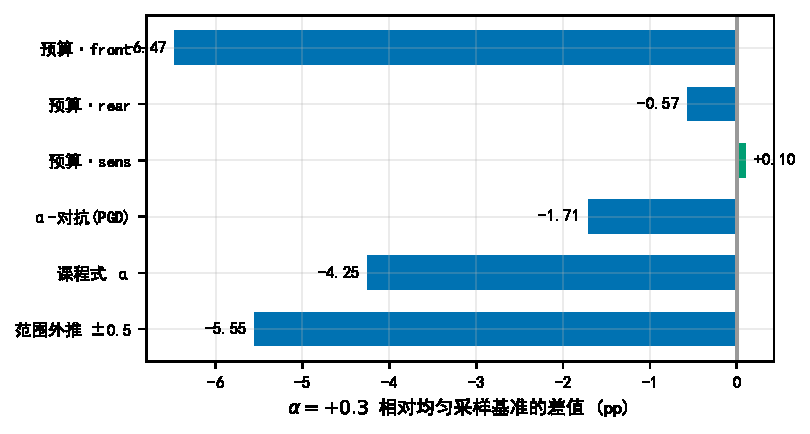
\includegraphics[width=0.70\textwidth]{F04_training_paths.pdf}
\caption{训练端的补救路径在 $\alpha=+0.3$ 上全部不优于均匀采样基准。
差值以基准（均匀采样，$\alpha=+0.3$ 时 26.03\%）为零线；
预算分配三种轮廓、$\alpha$ 空间对抗训练（PGD）、课程式采样、训练范围外推至 $\pm0.5$。
CIFAR-100 / SimpleCNN / 120 epoch / 单种子。
数据：\texttt{outputs\_cifar100/v3\_methods/*/alpha\_sensitivity.csv}。}
\label{fig:training}
\end{figure}

四条路径分别为：采样预算分配（三种轮廓，最好 26.13）、
$\alpha$ 空间对抗训练（24.32，$-1.71$）、课程式采样（21.78，$-4.25$）、
训练范围外推至 $\pm0.5$（20.48，$-5.55$）。没有一条超过基准。

其中最后一条最能说明问题的性质：\textbf{模型已经在 $\pm0.5$ 上训练过}，
但测试到 $\alpha=+0.5$ 时仍只有 2.71\%，同期负侧 $-$0.5 有 31.19\%，
相差 28.5 个百分点。正侧尾部不是采样覆盖问题，而是\textbf{结构性的不可训练区}。

这一边界不是"训练不够"造成的，而是"训练分布之外"造成的。
\cref{fig:extrapolation} 给出一个直接对照：把非线性感知训练的增益沿 $\alpha$ 轴外推，
正侧在 $\alpha\approx0.4$ 处归零并迅速转为劣势，
而负侧随外推距离\textbf{不降反升}。
也就是说，训练端手段的收益被它自己的训练分布框住；
这与 \cref{fig:training} 的四条路径互为印证。

\begin{figure}[t]
\centering
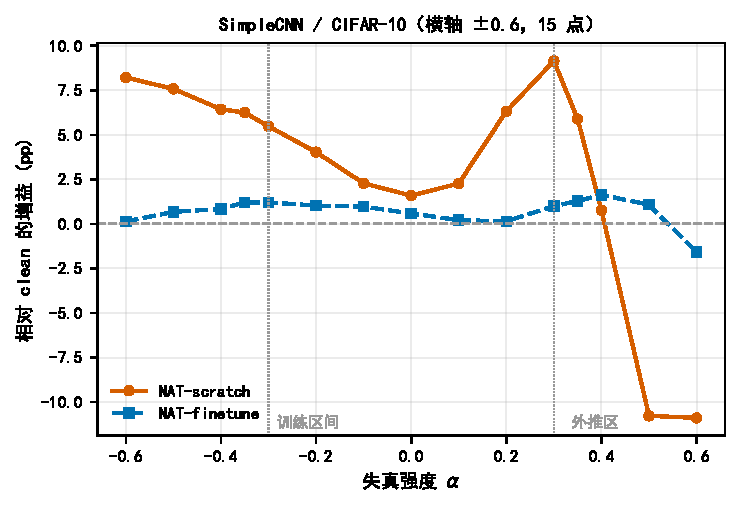
\includegraphics[width=0.70\textwidth]{F11_extrapolation.pdf}
\caption{非线性感知训练的收益是训练分布内的属性。
SimpleCNN 上两种训练策略相对干净模型的增益沿 $\alpha$ 轴的变化；
竖直虚线标出训练区间 $\pm0.3$，其外为外推区。
正侧在 $\alpha\approx0.4$ 处归零、$\alpha=+0.5$ 反转为 $-10.77$；
负侧在外推区保持正值并略有上升。
\textbf{注意：本图数据集为 CIFAR-10}（干净精度 84.90），
与正文其余各图的 CIFAR-100 不同，跨图不可直接比较绝对值。
数据：\texttt{outputs/extension4\_alpha\_wide/alpha\_wide\_scan\_summary.csv}。}
\label{fig:extrapolation}
\end{figure}

\subsection{损伤的形态是维度丢失，而不是类间距缩小}

既然信息还在（\cref{fig:probe}）而训练救不回（\cref{fig:training}），
损伤的形态是什么？\cref{fig:rank} 给出答案。

\begin{figure}[t]
\centering
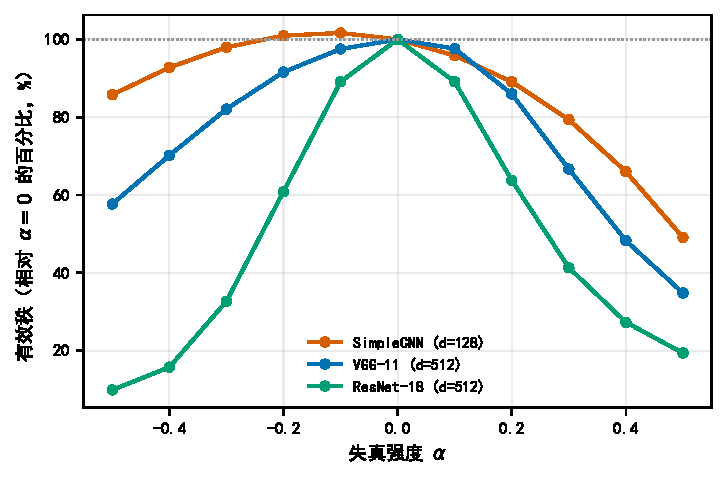
\includegraphics[width=0.70\textwidth]{F05_rank_collapse.pdf}
\caption{正侧失真使末端特征的有效秩塌陷，负侧几乎不动。
纵轴为按各模型 $\alpha=0$ 归一化后的有效秩（$\exp(-\sum p_i\ln p_i)$，$p_i$ 为归一化奇异值）；
横轴 11 个 $\alpha$ 点。三个主干的特征维数分别为 128 / 512 / 512。
数据：\texttt{outputs\_cifar100/v5\_rank\_collapse/rank\_stats*.csv}。}
\label{fig:rank}
\end{figure}

$\alpha=+0.3$ 时有效秩下降 20.6\%（SimpleCNN）、33.3\%（VGG-11）、58.7\%（ResNet-18）；
负侧同强度只降 2.0\% / — / —。
更关键的是，\textbf{同强度下正侧的 Fisher 判别比反而高于负侧}——
$\text{Fisher}(+\alpha)>\text{Fisher}(-\alpha)$ 在 $|\alpha|\in\{0.1,\dots,0.5\}$ 上\textbf{五点全成立}
（例如 $|\alpha|=0.3$ 时 0.45669 对 0.39062）。
类间可分性没有变差，丢失的是\textbf{维度}。

（\textbf{注意措辞}：这里说的是\textbf{跨正负的比较}，不是"正侧的 Fisher 随失真单调升高"——
沿正侧看它是\textbf{先升后降}的，只有 $\alpha=+0.1$ 那一点高于 clean
（0.50124 vs 0.49096），此后单调下降。上文早期版本写作"正侧失真下 Fisher 反而升高"，
丢了比较对象，是可被本文表格否证的错误表述，已更正。）
这与前文的幅度统计一致：$\alpha>0$ 把深层特征的幅度向中段压缩
（fc 与 conv1 的 L2 范数比从 0.45 降到 0.23），端点不变而中段被压低。

这就解释了"信息还在但训练救不回"这个表面矛盾：
信息仍存在于剩余的维度里，但这些维度在主干参数的可达域之外；
只有换一个读出才能在新的几何下重新找到判别方向。

\subsection{读出能拿回多少，由表征的秩损失决定}

如果上一节的机制成立，那么"秩掉得越多，读出能拿回的越少"应当成立。
\cref{fig:rankrec} 把三个容量档的秩损失与各自的读出恢复率配对。

\begin{figure}[t]
\centering
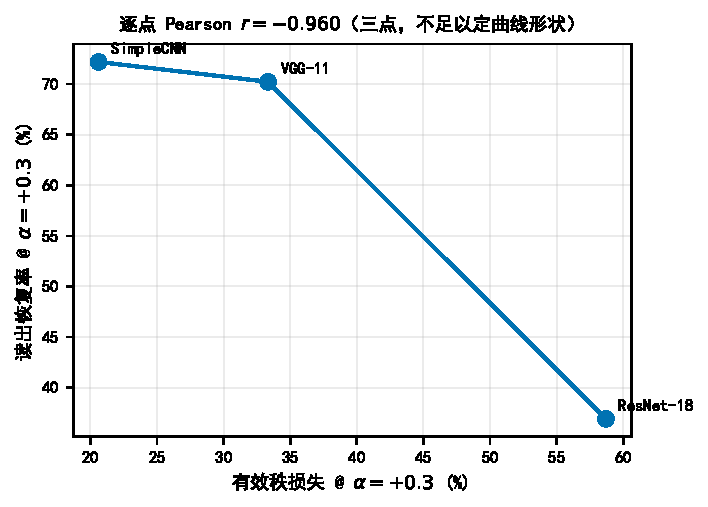
\includegraphics[width=0.58\textwidth]{F06_rank_vs_recovery.pdf}
\caption{秩损失与读出可恢复量的关系（三点）。
恢复率定义为读出适配在 $\alpha=+0.3$ 的精度除以同一读出文件里原始头在 $\alpha=0$ 的精度。
三点在 $\alpha=+0.3$ 上单调，逐点 Pearson $r=-0.960$。
\textbf{三点不足以定曲线形状}，形状提示为"先平后塌"。
数据：\texttt{rank\_stats*.csv} 与 \texttt{v3\_readout\_repair/*ep24*.csv}。}
\label{fig:rankrec}
\end{figure}

秩损失 20.6\% / 33.3\% / 58.7\% 对应恢复率 72.2\% / 70.2\% / 36.9\%（$r=-0.960$），趋势成立。
但反向不成立：ResNet-18 掉了 58.7\% 的秩，读出仍拿回 36.9\%
（相对自带头 6.22 仍有 $+20.60$），所以\textbf{塌陷不等于不可恢复}。
三点也定不了曲线形状——逐点看前两点只差 2.0 个百分点，第三点比第二点低 33.3，
更像"先平后塌"而非直线。这一点作为提示记录，需第 4 个容量档才能判定。

\subsection{池化密度是第二个独立杠杆，它的保护主要来自降维}

读出侧的杠杆要求读出层可写。有没有不依赖这一点的、纯架构的杠杆？
\cref{fig:maxpool} 给出一个零训练成本的答案。

\begin{figure}[t]
\centering
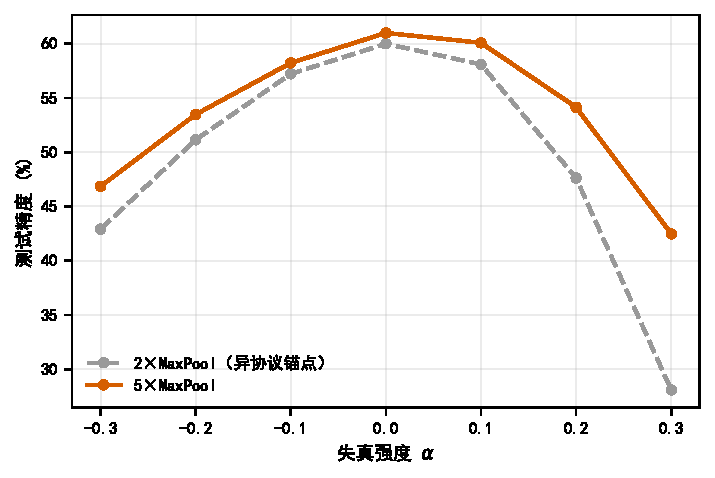
\includegraphics[width=0.70\textwidth]{F07_maxpool_density.pdf}
\caption{池化密度是独立的架构级杠杆。
把 SimpleCNN 的最大池化层从 2 个增加到 5 个——参数量不变、训练脚本不变、训练成本为零——
$\alpha=+0.3$ 从 28.09 提升到 42.47。
虚线为第一阶段 100 epoch 的产物，与实线的 120 epoch 不同协议，
仅作锚点、不参与同协议对比。
数据：\texttt{outputs\_cifar100/v3\_methods/simple\_cnn\_mp\_clean\_uniform/alpha\_sensitivity.csv}。}
\label{fig:maxpool}
\end{figure}

$\alpha=+0.3$ 从 28.09 提升到 \textbf{42.47}（干净训练）、26.03 到 \textbf{41.55}（鲁棒训练；
两侧同为逐层独立采样，同 seed 配对，增益 $+15.52$），
七点均值提升 4.5$\sim$4.9 个百分点，而干净精度不降。
增益与读出适配同级，但训练成本为零。

\textbf{保护从哪里来？} 三个候选机制被逐一检验，全部否证：

\begin{table}[t]
\centering
\caption{池化保护的三个候选解释与排除依据}
\label{tab:pool}
\small
\begin{tabular}{p{2.6cm}p{4.4cm}p{6.4cm}}
\toprule
候选解释 & 检验 & 结论 \\
\midrule
池化"吸收"了失真
& 归一化三次映射与 max 在非负域是否可交换
& 在池化输入（post-ReLU，非负）上\textbf{精确可交换}，$\max|\Delta|=$ 0.000e+00；
  但可交换却非成因——交换律成立时保护并未因此产生 \\[2pt]
质量向恒等区集中
& 5-pool 与 2-pool 的易感度 $S$ 与不变区占比
& 5-pool 的 $S$ \textbf{反而更高}（conv4：0.1527 vs 0.1134），
  不变区占比几乎不变 \\[2pt]
max 的选择性或可交换性
& 换成 top-2 池化（与 $f_\alpha$ 不可交换）
& 保护与 max 等同（42.98 vs 42.47，单种子） \\
\bottomrule
\end{tabular}
\end{table}

三条排除之后，唯一显著的差异是\textbf{空间元素数从 256 降到 16}。
进一步做同协议 3 种子对照：5$\times$max 的 \texttt{drop@0.3} 为 $20.60\pm1.54$、
5$\times$avg 为 $21.78\pm0.91$，差 $+1.17$。
该差值落在预登记的 1$\sim$2 个百分点区间（差值的标准误 1.03，$z\approx1.1$），
因此 \textbf{"降维 : 非均值聚合"的定量比例不予裁决}，只能给出方向性结论：
\textbf{保护主要来自降维}。

\subsection{两个杠杆在尾部可以叠加，且失真强度可以在线估计}

\cref{fig:maxpool} 的架构杠杆与 \cref{fig:readoutnat} 的读出杠杆是否互斥？
把两者叠（5$\times$MaxPool 主干 $+$ readout-NAT）后，$\alpha=+0.3$ 达 \textbf{49.12}，
比架构单独高 6.65、比读出单独高 5.74。两个杠杆在尾部近似正交可叠加。

部署时还有一个信息问题：现场并不知道失真有多强。
用读出层的特征做岭回归即可恢复它：在四个主干$\times$数据集组合上，
$R^2$ 为 \textbf{0.827$\sim$0.935}、MAE \textbf{0.036$\sim$0.061}，
$\hat{\alpha}$ 在 $\pm0.3$ 区间上近乎无偏。

\textbf{主干越深，估计越准}：VGG-11（Exp2 主干）$R^2=\textbf{0.9516}$ / MAE 0.0324，
ResNet-18（Exp3 主干）$R^2=\textbf{0.9778}$ / MAE 0.0219。
（出处：\texttt{outputs\_cifar100/v5\_full\_recipe/recipe\_robust\_*.csv} 的
\texttt{ridge\_R2} / \texttt{ridge\_MAE} 两列。）
这与直觉一致——深层特征的维度更高（512 对 128），承载的失真强度信息更完整；
而浅层里 MaxPool 会把一部分 $\alpha$ 信息压掉（$5\times$MaxPool 主干的 $R^2$ 为 0.8323，
低于无池化的 0.933）。

这意味着可以按估计值在多个头之间调度，且\textbf{在深层上这个调度信号比浅层更可靠}。

\subsection{门控能把读出的 clean 代价收回来——但有清晰的门槛}
\label{sec:gating}

读出适配付出了 3.19$\sim$6.67 个百分点的干净精度代价。
既然 $\alpha$ 可以估计，一个自然的做法是同时保留干净头与鲁棒头，
按 $w=\mathrm{clip}(|\hat{\alpha}|/0.3,\,0,\,1)$ 在两个头的 logits 之间插值。
\cref{fig:gating} 把七个 (代价, 红利) 点画在一起，结论与直觉相反。

\begin{figure}[t]
\centering
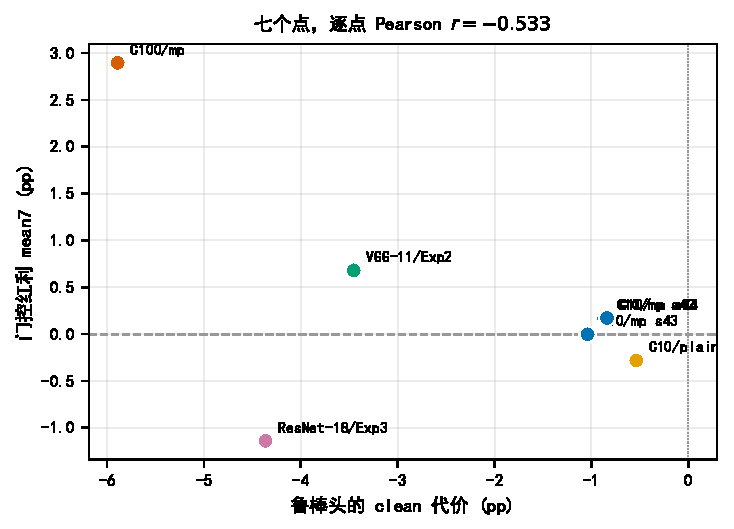
\includegraphics[width=0.70\textwidth]{F08_gating_benefit.pdf}
\caption{门控红利不随鲁棒头代价单调增长。
横轴为鲁棒头相对干净头在 $\alpha=0$ 的精度损失（负值=鲁棒头更差），
纵轴为门控相对单用鲁棒头在 \texttt{mean7} 上的增益。
七个点取自四个主干配置与两个数据集，各 3 个种子。
逐点 Pearson $r=-0.533$；去掉 CIFAR-100 远点后 $n=6$ 时符号反转为 $+0.351$。
数据：\texttt{v5\_full\_recipe/recipe*.csv}。}
\label{fig:gating}
\end{figure}

在 CIFAR-100/mp 上，鲁棒头的干净代价是 $-5.89$，门控收回 $+2.90$，
七个扫描点里有三个超过两头中较优者。
但当把深层主干加进来，代价落进了此前空白的 2$\sim$5 个百分点区间
（VGG-11 $-3.45$、ResNet-18 $-4.36$），\textbf{红利却没有跟着变大}：
分别是 $+0.68$ 与 $\mathbf{-1.14}$——在 ResNet-18 上门控比单用鲁棒头还差 1.14 个百分点。

原因在逐 $\alpha$ 曲线上看得很清楚：ResNet-18 的自带分类头在\textbf{负侧是崩的}
（$\alpha=-0.2$ 只有 10.27\%）。软门控按 $w=|\hat{\alpha}|/0.3$ 插值，
在真实 $\alpha=-0.2$ 处 $w\approx0.67$，于是三分之一权重的坏头把 45.64 拖到 39.21。
插值没有任何机制知道"其中一个头在这个 $\alpha$ 上是坏的"。

因此门控有效需要\textbf{两个前提同时成立}：
\begin{enumerate}[leftmargin=2em,itemsep=2pt]
  \item 鲁棒头的干净代价足够大（有东西可回收）；
  \item 两个头在整个 $\alpha$ 轴上都不能崩掉（否则插值会把一个头在该点的灾难带进来）。
\end{enumerate}

一个多数据集的自我检验值得一提。上述机制是在 CIFAR-100 上事后发现的。
为检验它，在\textbf{尚无任何配方结果}的 CIFAR-10 上锁定了全部超参、
并在跑之前写死了五条判据（C1--C5）。
结果：形式判据成立，但强主张\textbf{未复现}——
"插值超过 oracle"的判据由 3/7 降到 \textbf{1/7}%
\footnote{\textbf{但这个计数不稳健，本节的结论不挂在它上面。}
第七阶段复核发现：CIFAR-10 侧有一个 $\alpha$ 点的"软门控减 oracle"只有 $-0.0100$ pp
（$\alpha=-0.2$），而 CPU 与 CUDA 的\textbf{设备差异单独就能把它翻成 $+0.0033$}
——也就是说 \textbf{3/7 与 1/7 之差可以只由设备口径造成}。
（CIFAR-100 侧对应点的最小裕度是 0.1567 pp，是稳的。）
⇒ 本节的结论一律挂在\textbf{幅度}上，不挂在计数上。}，
门控相对 oracle 由 $+0.12$ 变成 $-0.07$，
门控红利由 $+2.90$ 缩到 $+0.17$。
复现的是\textbf{弱支配}（不差于任一头），不是集成增益。
机制因此被改写成更保守的形式：\textbf{门控红利 $=$ 鲁棒头干净代价的回收量}；
当干净代价小于 1 个百分点时，直接用单鲁棒头即可。

\textbf{再补一步：那个 $+0.17$ 的裕度是不是碰巧？}
上面的 CIFAR-10 检验只用了\textbf{一个主干种子}——3 个种子变的是鲁棒头与估计器，不是主干本身。
为判断裕度是否稳健，把 CIFAR-10 的 mp 主干补到 3 个种子，每个主干各跑一次完整配方：

\begin{center}
\small
\begin{tabular}{lcccc}
\toprule
主干种子 & mean7（干净头） & mean7（鲁棒头） & mean7（软门控） & $m$ \\
\midrule
42 & 82.68 & 85.02 & 85.19 & $+0.169$ \\
\textbf{43} & 82.19 & 84.90 & 84.90 & $\bm{-0.003}$ \\
44 & 82.61 & 85.00 & 85.17 & $+0.171$ \\
\bottomrule
\end{tabular}
\end{center}

（$m=\text{mean7}(\text{软门控})-\max(\text{mean7 干净头},\ \text{mean7 鲁棒头})$。
判据跑前写死：\textbf{任一 $m\le0$ 则 C1 改判"不可分辨"}。）

\textbf{主干种子 43 的 $m=-0.003$，判据命中} ⇒ C1 由"弱通过"改判
\textbf{"不可分辨"}，软门控在 CIFAR-10 上的定性定为\textbf{"与单头不可区分"}。
更准确的说法是：\textbf{差值在 $0\sim+0.17$ 之间飘，三个主干种子里有一个正好落在 0 上}
（平均 $+0.112$，全部远小于主干级的 mean7 噪声）。
\textbf{部署推荐不变}——CIFAR-10 一直推荐单鲁棒头。

\textbf{最后记一笔被替代掉的配置。}按本项目的纪律，预登记未达标的记录必须留下：
最早预登记的完整配方用的是\textbf{硬} $\tau$ 路由，端到端实测三项判据里
mean7 54.49（达标）、clean 60.92（达标）、但 $\alpha=+0.3$ = \textbf{47.90}（\textbf{未达标}，
阈值 48.5，差 0.60）。\textbf{软门控是在看到这次失败之后才引入的}——
这正是上文所有"事后变体"措辞的来源，也是为什么本文对它的每一个主张都要求跨数据集复现。

另外，门控的两前提\textbf{无法}做成装前的量化自检：
把"崩"定义为两头在 7 个 $\alpha$ 点上的最小精度，或定义为最坏相对缺口，
两种定义在已有的 7 个点上\textbf{都不分离}红利的符号
（VGG-11 的最小精度只有 15.73 却红利为正；CIFAR-10/mp 主干 43 的最小精度有 69.23 却红利为 $-0.003$）。
该判据作为事后机制解释保留，不作为预测规则。

\paragraph{部署时的失真分布会漂移——门控扛得住吗？}
上面所有比较都在训练分布 $U[\pm0.3]$ 上做。真实芯片的失真分布未必如此，
于是用六种分布重做同一套门控（主干为 $5\times$MaxPool 变体，权重不变，只换评估分布）：

\begin{center}
\small
\begin{tabular}{lccccc}
\toprule
评估分布 & clean 头 & robust 头 & 硬路由 & \textbf{软门控} & oracle \\
\midrule
① $U[\pm0.3]$（训练分布，参照） & 54.12 & 52.19 & 54.49 & \textbf{55.08} & 54.96 \\
② 仅正向 & 54.53 & 52.85 & 55.49 & \textbf{56.07} & 55.87 \\
③ 仅负向 & 55.43 & 52.25 & 55.10 & \textbf{55.50} & 55.56 \\
④ 双峰（$\pm0.2$ 各半） & 53.71 & 52.03 & 53.25 & \textbf{54.40} & 54.02 \\
⑤ 尾部集中（$\pm0.3$ 各半） & 45.63 & \textbf{48.57} & 48.10 & \textbf{49.11} & 48.57 \\
⑥ 单峰 $N(+0.3,0.05)$ & 44.51 & 49.08 & 48.57 & \textbf{49.83} & 49.24 \\
\bottomrule
\end{tabular}
\end{center}

两件事：

\textbf{(1) 软门控在 6/6 种分布下都是最好的}（其中 4 种超过 oracle）。
它不需要知道真实分布是什么——因为插值权重 $w=|\hat\alpha|/0.3$ 是\textbf{逐样本}算的，
分布的形状不影响它。

\textbf{(2) 硬路由在漂移下会退化}：在⑥以外的⑤（尾部集中）处，硬路由只有 48.10，
\textbf{反而低于单用鲁棒头的 48.57}。原因是硬路由在 $|\hat\alpha|$ 的阈值附近做二值选择，
而尾部集中时 $\hat\alpha$ 大量落在阈值两侧，选错的代价被放大。

\textbf{但这条红利不是无条件的}：同一组实验在\textbf{无池化}（plain）主干上做，
⑤ 处软门控 47.70 对鲁棒头 47.71 —— \textbf{红利消失}（$-0.01$）。
这与第 \ref{sec:gating} 节的边界条件一致：\textbf{软门控的价值取决于主干自身的尾部可用性}，
分布漂移只是让它更明显或更不必要。

\subsection{失真与量化联合作用时，低位量化在池化密集架构上会反转成增益}

真实芯片在模拟域失真之外还有 ADC 量化。两者同时存在时相互放大还是抵消？
\cref{fig:dithering} 给出一个反直觉的答案。

\begin{figure}[t]
\centering
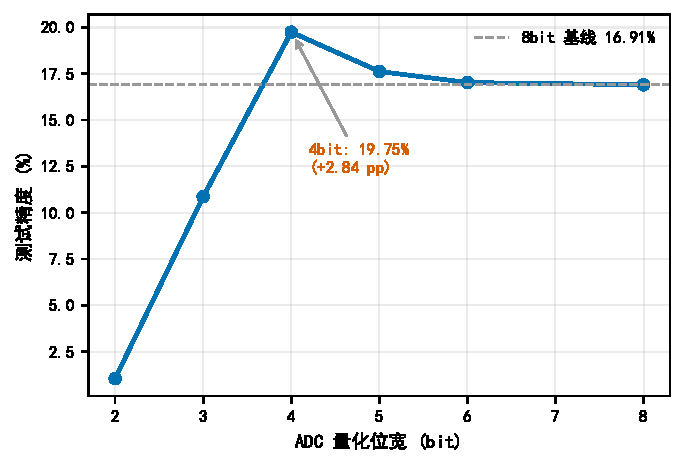
\includegraphics[width=0.62\textwidth]{F10_dithering.pdf}
\caption{低位量化在池化密集架构上反转成增益。
VGG-11、固定 $\alpha=+0.3$、CIFAR-100，扫描 ADC 位宽；
虚线为 8 bit 基线。4 bit 时精度最高，比 8 bit 高 2.84 个百分点。
数据：\texttt{outputs\_cifar100/extension5\_dithering\_vgg11/group\_a\_bits\_scan.csv}。}
\label{fig:dithering}
\end{figure}

在 VGG-11（5 个 MaxPool）上，4 bit 量化的精度\textbf{高于} 8 bit（CIFAR-100：$+2.84$；
CIFAR-10：$+6.53$）。三个候选假设通过剂量匹配的三组对照、样本级翻转统计与激活分布统计判决：

\begin{itemize}[leftmargin=2em,itemsep=2pt]
  \item \textbf{H1 随机去相关 —— 否决}。用与 4 bit 等效剂量的纯高斯/均匀噪声替代量化，
        精度不升反降（$-2.45$ / $-1.87$）；8 bit 基线上叠加最优剂量噪声的增益为 $-0.03$。
        样本级翻转统计给出三个量级的反差：4 bit 的救回:杀死为 4.15:1（净 $+653$ 样本），
        而噪声条件约为 1:1（净 $+7$ / $-19$）。
  \item \textbf{H2 分布重塑 —— 确认（核心机理）}。分类器输入分布的峰度在失真下从 1.486 被压平到 0.110，
        4 bit 的粗离散化把它恢复到 \textbf{0.214}，部分重建可分性。
        存在甜点带：3 bit 峰度更高（0.384）但精度略降（重塑过头叠加信息损失），
        2 bit 信息量不足、峰度与精度双双坍缩。
  \item \textbf{H3 MaxPool 交互 —— 支持（必要条件）}。无 MaxPool 的 ResNet-18 完全免疫（$+0.39$）；
        但只有 2 个 MaxPool 的 SimpleCNN 是\textbf{负增益}（$-13.68$）。
        因此 MaxPool 是必要而非充分条件，其密度决定量化误差是被修正还是被放大。
\end{itemize}

这条结果对"数字域后处理能救多少"给出了分层答案：
同一个 4 bit ADC，在池化密集架构上是补偿，在池化稀疏架构上是负担。

\subsection{为一种失真做的鲁棒性训练，不会顺带保护另一种}

前九节讨论的都是同一类扰动：确定性的、输入相关的非线性失真。
现实中的模拟域还有另一类误差源——零均值、与信号无关的\textbf{加性随机噪声}。
一个自然的问题是：\textbf{为其中一种训练出的鲁棒性，能不能迁移到另一种？}
如果不能，那么两类误差必须分别对待；如果能，联合训练就够。

\paragraph{迁移：近正交，但幅度依赖架构。}
把一条通路上训好的权重拿到另一条通路上扫，测"扰动敏感性"的变化幅度
$\max|\Delta_\sigma|$（超过 1.2 个百分点判为非零迁移）：

\begin{center}
\small
\begin{tabular}{llc}
\toprule
架构 & 配方对 & $\max|\Delta_\sigma|$ \\
\midrule
SimpleCNN & Exp2（校准）vs 原始 & 1.16 \\
SimpleCNN & NAT-scratch vs clean & 2.43 \\
SimpleCNN $+$ 3$\times$MaxPool & NAT vs clean & 0.98 \\
\textbf{VGG-11} & \textbf{Exp2（校准）vs clean} & \textbf{5.26} \\
ResNet-18 & Exp2（校准）vs clean & 1.41 \\
\bottomrule
\end{tabular}
\end{center}

⇒ 「两通路正交、迁移为零」这条结论\textbf{是架构依赖的}：
在 SimpleCNN 与 ResNet-18 上成立（$\le$1.41），
但在 \textbf{MaxPool 密集的 VGG-11 上被打破}（5.26）。
值得注意的是，加三个 MaxPool 反而\textbf{降低}了迁移（2.43 $\to$ 0.98），
所以"MaxPool 密度"本身不是迁移的成因——更可能是校准模块作用于空间特征图的方式（\S\ref{sec:related} 的讨论）。

\paragraph{训练端：不是零迁移，而是\textbf{单向强干扰}。}
迁移幅度小，容易被读成"两者互不影响"。但训练端的对照否证了这个读法。
在同一个 harness 上做 $2\times2$（是否注入 $\alpha$ $\times$ 是否注入 $\sigma$）：

\begin{center}
\small
\begin{tabular}{lcccc}
\toprule
训练条件 & clean & $\alpha=+0.3$ & $\sigma=0.30$ & 双扰动最坏点均值 \\
\midrule
无训练（clean 模型） & 59.99 & 28.09 & 3.98 & 16.04 \\
$\alpha$-only & \textbf{60.85} & 26.03 & 4.40 & 15.22 \\
$\sigma$-only & 55.79 & 22.01 & \textbf{27.19} & \textbf{24.60} \\
$\alpha+\sigma$（联合） & 55.20 & 15.27 & \textbf{31.31} & 23.29 \\
\bottomrule
\end{tabular}
\end{center}

三件事同时成立：

\textbf{(1) $\alpha$ 训练对 $\sigma$ 几乎零收益}（4.40 vs 3.98）——这一侧确实是正交的。
\textbf{(2) 但 $\sigma$ 训练使 $\alpha$ 侧付出代价}：$\alpha=+0.3$ 从 28.09 掉到 22.01（$-6.08$），
干净精度也掉 4.20。联合训练更糟：$\alpha$ 侧 15.27
（相对 clean 模型 $-12.82$，相对只做 $\alpha$ 训练的 26.03 又低 $-10.76$）。
\textbf{(3) 双扰动并存时的最优配方是 $\sigma$-only，不是联合训练}：
joint 里的 $\alpha$ 注入是\textbf{净负担}——它在 $\sigma$ 侧只多拿 4.12，
却付出 $\alpha$ 侧 $-6.74$。

⇒ 正确表述不是"两条通路正交"，而是「\textbf{迁移近正交，但训练端存在单向强干扰}
（$\sigma\to\alpha$ 有代价、$\alpha\to\sigma$ 无收益）」。

\paragraph{这条结论的工程含义。}
如果部署环境同时存在两类误差，\textbf{不应把两种扰动一起塞进训练}——
应该先显式训 $\sigma$ 鲁棒性（它是必须显式训练的，且收益大：$\sigma=0.3$ 处 3.98 $\to$ 27.19），
然后\textbf{在读出侧}单独处理非线性失真（第 \ref{sec:probe} 节的方法正好不碰主干，
因此不会与 $\sigma$ 训练互相干扰）。
换言之，本节的结论与本文的主线是一致的：
\textbf{训练端做的事越少越好，剩下的交给读出。}

\subsection{这些效应有多大：用错协议会把方差估高六倍}
\label{sec:variance}

上面所有差值都需要一个误差尺度。本文的方差标定给出两个数值，其中一个足以改变结论。

\textbf{第一，尾部指标的种子方差远大于干净精度。}
同协议实测：浅层鲁棒训练尾部 $\pm0.39$、架构变体 $\pm0.95\sim1.58$、
深层读出 $\pm3.18\sim3.40$；而同组的干净精度只有 $\pm0.07\sim1.85$。
更麻烦的是干净精度\textbf{不能外推}：ResNet-18 按 2 个种子报的 $\pm0.15$
在补上第 3 个种子后变成 $\pm1.85$（第 3 个种子的干净精度为 67.61，
比另两个高 2.6$\sim$4.1 个百分点）。三个容量的干净方差跨度达 26 倍。

\textbf{第二，混用协议会把方差估高约 6 倍。}
一组 3 seed 的鲁棒训练尾部读数，若三个种子来自两个脚本，
标准差是 $\pm2.561$；补跑同脚本的第三个种子后，同协议标准差只有 $\pm0.392$。
进一步的定量分解显示，那 2.56 里绝大部分\textbf{不是随机噪声，而是两种训练配方之间的系统差}
（组内两个数相差 5.32，与实测的脚本级处理效应 5.52 几乎相等）。
也就是说，把处理效应误读成了噪声。

\textbf{第三，也是最难处理的一条：跨训练实现的精度数字不可移植。}
两个脚本（记为 A 与 B）在数据加载、归一化、优化器、batch、epoch、调度器、
增强、钩子机制、采样位置与评估口径上逐项一致，
同 seed 的逐 epoch 训练损失全程贴合（差 $\le0.016$，无分叉），
但 A 训出的鲁棒权重尾部稳定落在 $21.03\pm1.00$，
B 训出的\textbf{六个} run 全部落在 $26.58\pm0.29$，两者相差 \textbf{5.55} 个百分点（$z=9.4$）。

为定位原因做了三次独立的干预，全部失败：

\begin{figure}[t]
\centering
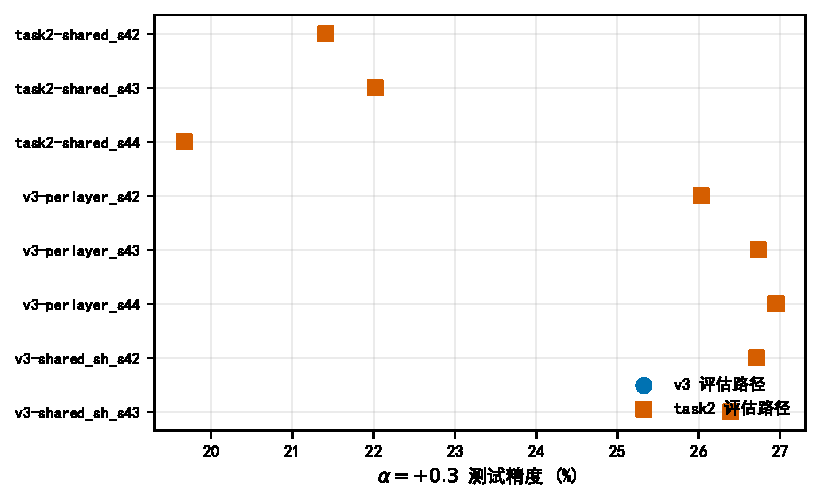
\includegraphics[width=0.72\textwidth]{F09_crosspath.pdf}
\caption{交叉评估：差异不在评估路径。
把 8 个权重分别在另一脚本原样导入的评估函数下重扫，
两条路径给出\textbf{逐位相同}的读数（含干净精度）；
但两组权重稳定分成两簇（A 脚本 19.7$\sim$22.0，B 脚本 26.0$\sim$27.0）。
数据：\texttt{outputs\_cifar100/v6\_p4e\_crosspath/crosspath.csv}。}
\label{fig:crosspath}
\end{figure}

\begin{table}[t]
\centering
\caption{5.55 个百分点差异的三次归因尝试与结果}
\label{tab:mystery}
\small
\begin{tabular}{p{2.4cm}p{3.6cm}p{8.2cm}}
\toprule
轮次 & 当时的归因 & 结果 \\
\midrule
1 & 尾部\textbf{种子噪声} $\pm3.1$
& \textbf{否证}。三个种子来自两个脚本，同协议下标准差只有 $\pm0.39$；混协议把方差估高约 6 倍 \\[2pt]
2 & $\alpha$ 采样\textbf{粒度}（每批共享 vs 逐层独立）
& \textbf{否证}。在同一脚本内只切换粒度：26.55 vs 26.57，差 $+0.02$（$z=0.08$）；
  而同粒度跨脚本差 $+5.52$（$z=9.4$）。效应跟着脚本走，不跟着粒度走 \\[2pt]
3 & 随机数\textbf{消耗位置}（每批消耗 1 个 vs 5 个随机数）
& \textbf{否证}。同脚本把消耗数从 5 改成 1：26.66 vs 26.55，差 $+0.11$ \\
\bottomrule
\end{tabular}
\end{table}

已排除的解释累计为：种子噪声、$\alpha$ 采样粒度、随机数消耗数、
评估路径（\cref{fig:crosspath}，8 个权重 $\times$ 2 条路径逐位相同）、
训练动力学（逐 epoch 损失差 $\le0.016$）。
\textbf{该差异仍未归因，按已知未知记录。}

这条结论的实践含义是硬的：\textbf{部署校准必须与部署训练同实现、同路径}；
跨实现引用精度数字——包括与文献对比——都是无效的。

\paragraph{一个更实用的刻度：三级可分辨性。}
上面那条"跨实现不可移植"是一个\textbf{已知未知}，无法直接当门槛用。
但它旁边有两级\textbf{可以测准}的散布，合起来给出一个可操作的判断尺度：

\begin{center}
\small
\begin{tabular}{llc}
\toprule
层级 & 变的是什么 & 实测幅度 \\
\midrule
① 种子噪声 & 同一过程重复 & 尾部 $\pm0.39\sim3.40$；clean $\pm0.07\sim1.85$ \\
\textbf{② 过程自由度} & \textbf{同数据、同特征、同架构，只换拟合过程} & \textbf{3.45 pp} \\
③ 跨实现 & 同超参同种子，实现不同 & 5.55 pp（\textbf{未归因}）\\
\bottomrule
\end{tabular}
\end{center}

第 ② 级是这样测的：在\textbf{同一批冻结特征}上训同一个线性头，只换六种拟合过程
（sklearn 的 lbfgs / saga；torch 的 Adam 在 50 / 150 / 400 轮；SGD+动量 150 轮），
$\alpha=0$ 与 $+0.3$ 上各跑一遍。结果：

\begin{center}
\small
\begin{tabular}{lcccccc}
\toprule
拟合过程 & sklearn lbfgs & sklearn saga & Adam 50 & Adam 150 & Adam 400 & SGD+mom 150 \\
\midrule
$\alpha=0$ & 53.22 & 54.91 & \textbf{56.31} & 54.89 & \textbf{52.85} & 53.27 \\
$\alpha=+0.3$ & 48.25 & 50.75 & \textbf{51.57} & 50.37 & 48.55 & \textbf{48.12} \\
\bottomrule
\end{tabular}
\end{center}

⇒ \textbf{极差 $\Delta_{\text{proc}} = 3.45\sim3.46$ pp。} 同数据、同特征、同架构、同一个线性头，
\textbf{只换"怎么把它拟合出来"，就能差 3.45 个百分点。}

\textbf{这里有一个反直觉的细节值得单独记}：$\alpha=0$ 的最大值与最小值
\textbf{都来自同一个优化器的不同轮数}（Adam 50 轮最高 56.31、Adam 400 轮最低 52.85）。
⇒ \textbf{过程自由度的主要来源是"训多久"，不是"用哪个"。}
（$\alpha=+0.3$ 的最小值出自 SGD+动量，但最大值同样出自 Adam 50 轮。）

\textbf{由此得到一条判断规则}：任何"读出类"效应（换头、加正则、改容量）的可分辨门槛
\textbf{必须同时以 $\Delta_{\text{proc}}$ 为参照，不能只用种子噪声}——
因为种子噪声测的是"同一过程重复"的散布，而 $\Delta_{\text{proc}}$ 测的是"换一个过程"的散布，
\textbf{后者才是接收端口真正面对的那种不确定性}。
本文第 \ref{sec:gating} 节关于门控增益的每一个比较，其效应量都远大于种子噪声，
但与 $\Delta_{\text{proc}}$ 同量级——这一点读者在解释那些差值时应当一并考虑。

\section{讨论}
\label{sec:discussion}

\subsection{为什么修复的对象不是参数而是解码}

把 \cref{fig:probe}、\cref{fig:readoutnat}、\cref{fig:training} 三条并置：
信息仍在（探针可线性取用）、换读出即取到（尾部 $+13\sim23$）、
而参数空间的四条路径全部无效。这三条单独看都可以被别的解释吸收——
探针可能过强、"训练不够久"、读出适配可能是再分配——但并置之后"再分配"这个解释被排除，
因为分布式读出适配在每个扫描点都不显著劣化。

常规对抗鲁棒性的直觉是"扰动在参数空间里被吸收"：对抗训练之所以有效，
是因为训练分布覆盖了测试分布。但本文的扰动性质不同——它是确定性的、输入相关的系统误差，
逐层累积且与信号幅度挂钩。\cref{fig:rank} 表明这类误差不摧毁信息，
它改变信息的\textbf{几何}：把深层表征的有效秩压下去，而 Fisher 判别比在正侧反而高于同强度的负侧。
在一个丢维度的子空间里，"把参数训得更适应"不会增加维度；
换一个读出却可以在剩余的维度里重新找到判别方向。
\cref{fig:rankrec} 把这个直觉接上了定量：可恢复量随秩损失单调下降。

\subsection{一个可迁移的测量顺序}

更一般地，当失真同时具有"确定性、逐层累积、且权重不可重训"三个性质时，
\textbf{鲁棒性的杠杆位置由信息在哪一层被破坏决定，而不是由"哪一层参数多"或"哪一层最脆弱"决定}。
这条原理的可迁移形式是一个测量顺序，而不是一个方法：

\begin{enumerate}[leftmargin=2em,itemsep=2pt]
  \item \textbf{先测 headroom}：在冻结主干的末端特征上重训线性探针，与自带头比较。
        headroom 小 $\to$ 信息真的没了，只能动表征，回到常规鲁棒训练；
        headroom 大 $\to$ 杠杆在读出，训练端的投入大概率是浪费。
  \item \textbf{若杠杆在读出，再测秩损失}：它给可恢复量一个上界提示
        （本文：秩损失 20$\sim$59\% 对应恢复率 72$\sim$37\%）。
  \item \textbf{再看架构端有没有零成本的降维空间}（本文：池化密度）。
\end{enumerate}

本文给出 headroom 的两个对照值，说明第一步本身有区分力：
非线性失真 $+20.26$、加性高斯噪声 $+7.50$。
随机扰动与确定性系统误差在这个量上清楚地分开——
前者需要的是表征层面的平滑，后者需要的是解码层面的重定向。

\subsection{若要落到真实器件的数字后端}
\label{sec:deploy}

本节把上面的结论映射到存内计算的实际约束上：模拟阵列负责乘累加、权重\textbf{固化}，
阵列输出经 ADC 回到数字域，失真发生在模拟域的输入侧。
判定分三档——\textbf{可行} / \textbf{需改动} / \textbf{不可行}：

\begin{center}
\small
\begin{tabular}{p{3.0cm}p{2.0cm}p{9.4cm}}
\toprule
组件 & 判定 & 依据 \\
\midrule
\textbf{读出适配} & \textbf{需改动}
& 要求读出层位于数字域、或阵列里那一小块可重写。读出层只占全模型参数的
  \textbf{5.04\%}（SimpleCNN）/ \textbf{0.55\%}（VGG-11），挪出阵列对面积影响很小 \\[2pt]
\textbf{在线 $\alpha$ 估计} & \textbf{可行}
& 一次 $d$ 维点积（$d=128/512$），算力占主干前向的 \textbf{3.8e-4\%} / 2.4e-4\% \\[2pt]
\textbf{软门控} & \textbf{可行}（前提同第一条）
& 数字域逐元素运算，每次推理约 \textbf{400} 次操作；
  干净头是冻结不动的那一个，正好可以固化在 ROM 里 \\[2pt]
\textbf{冻结主干} & \textbf{可行}
& 就是"不训练主干"，天然符合权重固化 \\[2pt]
\textbf{MaxPool 密集主干} & \textbf{设计阶段零成本} / 部署后不可行
& 它是网络\emph{定义}的改动，只能在投片前决定；好消息是它零训练成本 \\[2pt]
\textbf{全网络重训} & \textbf{不可行}
& 阵列权重是烧录/固化的；而且训练端的四条路本来就救不了尾部（第 \ref{sec:limit} 节）\\
\bottomrule
\end{tabular}
\end{center}

\noindent\textbf{推荐的落地顺序}（三步，前两步都有实测支撑）：

\begin{enumerate}[leftmargin=2em,itemsep=2pt]
  \item \textbf{架构端先上}：MaxPool 密集主干。零训练成本，尾部 $+14.38$ 个百分点——
        但它只能在\emph{投片前}决定，所以这一条要最先定。
  \item \textbf{读出端再训}：$\alpha$-混合鲁棒头（24 epoch，约 12 分钟）。尾部再抬升一截，
        代价是干净精度下降——\textbf{代价的大小决定了第三步要不要做}。
  \item \textbf{门控按需加}：仅当鲁棒头的干净代价足够大时（CIFAR-100 式细粒度任务，
        代价 $-5.89$）才加，且\emph{先查两个头的逐 $\alpha$ 曲线}（第 \ref{sec:gating} 节的前提②）。
        代价 $\lesssim$1 pp 时直接用单鲁棒头。
\end{enumerate}

\textbf{一个必须说清的结构性前提}：以上全部依赖\textbf{读出层可写}。
若某款 CIM 把读出层也固化在阵列里，本方法整体不成立——
这不是精度问题，是可行性问题，因此它出现在第 \ref{sec:limit} 节的第一条局限里。

\noindent\textbf{本节的边界}：以上是\textbf{推演}，不是实测。
没有硬件实测、没有 RTL 或功耗仿真、也没有写出"读出层挪到数字域"的接口约定
（时序、位宽、与 ADC 的对接）。面积、延迟、功耗的绝对值本文没有算过。

\subsection{打开的问题空间}

\begin{enumerate}[leftmargin=2em,itemsep=2pt]
  \item \textbf{秩损失到可恢复量的曲线是什么形状？} 三点提示"先平后塌"，
        但三点定不了形状。这直接影响能否把可恢复量写成一个由秩损失预测的上界。
  \item \textbf{若失真形态不是三次多项式，headroom 还剩多少？} 高斯对照给了下界；
        更高阶、带温度漂移或器件失配的形态族未测。
  \item \textbf{读出侧杠杆的上界在哪？} 当前读出适配距探针给出的线性可达上界仍差约 4 个百分点，
        这个缺口是优化不足还是结构性的，未系统测量。
  \item \textbf{多头扩展}：把 $\alpha$ 与噪声强度 $\sigma$ 同时估出来、三头调度，
        是否优于单训 $\sigma$ 的配方？（本文的联合扰动数据已显示 $\sigma$-only 最优、
        $\alpha$ 注入是净负担，但未做三头路由。）
\end{enumerate}

\section{局限与未来工作}
\label{sec:limit}

以下几项限制各自导致了一个由本文发现引出的重要问题处于未决状态。

\textbf{(1) 失真模型是参数化假设，且无硬件实测。}
全部收益都测在 \cref{eq:distortion} 这一族上。若真实 CiM 的非线性更接近高阶多项式、
带温度依赖、或器件间失配有随机成分，headroom 还有多大、读出杠杆是否成立，本文无法回答。
已知的下界来自高斯对照（headroom 从 20.26 降到 7.50）。
\textbf{下一步}：结合真实 CiM 宏的实测特性标定失真参数，在形态族上重测 headroom。

\textbf{(2) 深层主干是单次训练产物。}
VGG-11 与 ResNet-18 的主干各只训了一次；读出侧的 3 个种子只反映读出训练的数据顺序与采样随机性，
不含主干训练方差。而深层上已知的方差已经不小（固定主干换读出种子，干净精度从 63.54 摆到 67.61）。
因此涉及深层的所有差值——包括 \cref{fig:gating} 上 ResNet-18 的 $-1.14$——
\textbf{是否在主干种子方差内无法裁决}。\textbf{下一步}：每个深层主干重训 2 个种子（约 16 小时）。

\textbf{(3) 池化保护的定量分解没有定下来。}
同协议 3 种子下 avg 与 max 的差值只有 $+1.17$，落在 1$\sim$2 个百分点区间，
差值的标准误 1.03（$z\approx1.1$）。本文只能给出方向（保护主要来自降维），
无法裁决"降维 : 非均值聚合"的比例。这条路的根本瓶颈是 avg 与 max 本身的差距太小。
\textbf{下一步}：换效应量更大的对照（池化窗口 $2\times2$ vs $4\times4$，或池化层的位置分布），
或补到 $\ge8$ 个种子每组。

\textbf{(4) 秩-恢复关系只有三个点}（见 \cref{fig:rankrec}）。
\textbf{下一步}：补第 4 个容量档。

\textbf{(5) 跨实现的 5.55 个百分点差异未归因}（\cref{tab:mystery}）。
已验证无效的路径是换评估路线；必须动训练循环。
\textbf{下一步}：逐行对齐两个训练循环做二分。

\textbf{(6) 读出适配要求读出层可写，且本文未评估其硬件代价。}
读出层占全模型参数的 5.04\%（SimpleCNN）/ 0.55\%（VGG-11），
结构条件是"读出层位于数字域或可重写"。
但面积、延迟、功耗的真实代价需要 RTL 或流片验证，超出本文范围。
若某款 CiM 把读出层也固化在阵列里，本文的方法整体不成立。

\section{结论}

在逐层三次多项式非线性失真下，神经网络在灾难尾损失的是读出的可解码性而非表征中的信息
（headroom 20.26 个百分点，而同一探针在高斯噪声下只有 7.50）。
这一诊断直接给出了修复路径：冻结全部模拟权重、只重训最后的线性层，
在三个主干上把 $\alpha=+0.3$ 提升 13$\sim$23 个百分点，
成本为主干重训的 1/15$\sim$1/30，并一致超过所有全网络鲁棒训练配方；
而训练端的四条补救路径全部失效。
架构端的池化密度提供一个与之正交的零成本杠杆（$+14.38$ 个百分点），
其保护主要来自降维。两个杠杆在尾部可叠加。
失真强度可由岭回归在线恢复，使门控可以逼近 oracle，
但门控有效需两个前提同时成立，其边界由本文给出。
最后，本文报告一条方法学结论：同一份权重在两条评估路径下读数逐位相同，
而不同训练脚本产出的权重稳定相差 5.55 个百分点且原因未明——
\textbf{精度数字不可跨训练实现移植}。

\appendix
\section{关键数值汇总}

\begin{table}[h]
\centering
\caption{本文引用的主要数值与出处}
\footnotesize
\setlength{\tabcolsep}{4pt}
\begin{tabular}{lll}
\toprule
数值 & 取值 & 出处 \\
\midrule
探针 headroom @$+0.3$（非线性 / 高斯） & $+20.26$ / $+7.50$ & \texttt{v7\_probe\_audit/ra\_onprotocol\_main.csv}（全量 10k 口径；旧 8k 为 $+20.12$/$+7.00$） \\
读出适配 @$+0.3$（三主干，3 seed） & 43.31 / 47.79 / 26.82 & \texttt{v3\_readout\_repair/*ep24*.csv} \\
全网络鲁棒训练 @$+0.3$（最好） & 26.57 / 24.69 / 6.22 & 台账 §13.12 / §9.7 \\
池化密度 $2\to5$ @$+0.3$ & 28.09 $\to$ 42.47 & \texttt{simple\_cnn\_mp\_clean\_uniform/} \\
有效秩损失 @$+0.3$（三主干） & 20.6\% / 33.3\% / 58.7\% & \texttt{v5\_rank\_collapse/rank\_stats*.csv} \\
秩损失 $\to$ 恢复率（三点，$r$） & $-0.960$ & 同上一行 + \texttt{v3\_readout\_repair/} \\
池化同协议 3 seed 差（avg$-$max） & $+1.17$（SE 1.03） & 台账 §13.8 \\
门控红利（C100/mp） & $-5.89 \to +2.90$ & \texttt{recipe\_simple\_cnn\_mp.csv} \\
门控红利（ResNet-18/Exp3） & $-4.36 \to -1.14$ & \texttt{recipe\_robust\_resnet18\_exp3resnet18.csv} \\
$\alpha$ 估计器（6 组：4 浅 2 深） & $R^2$ 0.827$\sim$0.978 & \texttt{v5\_full\_recipe/recipe*.csv} \\
Dithering 增益（C100 / C10） & $+2.84$ / $+6.53$ & \texttt{extension5\_dithering\_vgg11/} \\
跨实现尾部差 & $5.55$（$z=9.4$） & 台账 §14.6 \\
同协议方差 / 混协议方差 & $\pm0.392$ / $\pm2.561$ & 台账 §13.10 \\
\bottomrule
\end{tabular}
\end{table}

\begin{thebibliography}{99}
\bibitem{cim_survey} Yu S, Chen P Y. Emerging memory technologies: recent trends and prospects[J]. IEEE Solid-State Circuits Magazine, 2016, 8(2): 43--56.
\bibitem{puma} Ankit A, El Hajj I, Chalamalasetti S R, et al. PUMA: a programmable ultra-efficient memristor-based accelerator for machine learning inference[C]//ASPLOS. Providence: ACM, 2019: 715--731.
\bibitem{nat} Zhu M, Liu Y, Wang Z, et al. Nonlinearity-aware training for accurate and robust compute-in-memory neural networks[J]. IEEE TCAD, 2022, 41(11): 3961--3973.
\bibitem{quant} Jacob B, Kligys S, Chen B, et al. Quantization and training of neural networks for efficient integer-arithmetic-only inference[C]//CVPR. Salt Lake City: IEEE, 2018: 2704--2713.
\bibitem{dither} Wannamaker R A, Lipshitz S P, Vanderkooy J, et al. A theory of nonsubtractive dither[J]. IEEE Transactions on Signal Processing, 2000, 48(2): 499--516.
\bibitem{resnet} He K, Zhang X, Ren S, et al. Deep residual learning for image recognition[C]//CVPR. Las Vegas: IEEE, 2016: 770--778.
\bibitem{vgg} Simonyan K, Zisserman A. Very deep convolutional networks for large-scale image recognition[C]//ICLR. San Diego: ICLR, 2015: 1--14.
\bibitem{cifar} Krizhevsky A. Learning multiple layers of features from tiny images[R]. Toronto: University of Toronto, 2009.
\bibitem{lpft} Kumar A, Raghunathan A, Jones R, et al. Fine-tuning can distort pretrained features and underperform out-of-distribution[C]//International Conference on Learning Representations. 2022. arXiv:2202.10054.
\bibitem{mtjcal} Xiao Z, Naik V B, Lim J H, et al. Adapting magnetoresistive memory devices for accurate and on-chip-training-free in-memory computing[J]. Science Advances, 2024, 10(38): eadp3710.
\bibitem{gjepa} Rabby G, Auer S. When Graph-JEPA learns the wrong thing: diagnosing and repairing category-conditional collapse[R]. 2026. arXiv:2608.20516.
\end{thebibliography}

\end{document}
